%Dokumentinnstillinger:---------------------------------
%Ved å google flitting kan du finne ut hva de forskjellige tingene her betyr, og hvordan du kan gjøre eventuelle endringer.
\documentclass[a4paper,11pt,norsk]{article}
\usepackage[utf8]{inputenc}
\usepackage{a4wide}
\usepackage{lmodern}
\usepackage[T1]{fontenc}
\usepackage{babel}
\setlength{\parindent}{0pt} 
\setlength{\parskip}{2ex}
\usepackage{fixltx2e}
\usepackage{amsmath}
\usepackage[pdftex, pdfborderstyle={/S/U/W 0}]{hyperref}
\usepackage{graphicx}
\usepackage[font=small,labelfont=bf]{caption}
\usepackage{tabularx}
\usepackage{multirow}
\usepackage{float}
\usepackage{mathtools}
\usepackage{siunitx}
\usepackage{hyperref}
\usepackage{pdfpages}

\begin{document}

%Headingdel:---------------------------------------------
\begin{minipage}[c]{0.15\textwidth}

\includegraphics[width=2.0cm]{elsys_pos_staaende_ntnu}  
\end{minipage}
\begin{minipage}[c]{0.85\textwidth}

\renewcommand{\arraystretch}{1.7}
\large 
\begin{tabularx}{\textwidth}{|X|X|}
\hline
\multicolumn{2}{|l|}{} \\
\multicolumn{2}{|l|}{\huge \textbf{Designnotat}} \\
\multicolumn{2}{|l|}{}  \\
\hline
\multicolumn{2}{|l|}{Tittel: 
%Skriv inn tittel her:------------------------------------------
Frekvensdobbler
} \\
\hline
\multicolumn{2}{|l|}{Forfattere: 
%Skriv inn forfattere her:--------------------------------------
Morten Klingan Hovstad
} \\
\hline
%Skriv inn versjon og dato her her:-----------------------------
Versjon: 1.0 & Dato: 27.03.22
\\
\hline 
\end{tabularx}
\end{minipage}
\normalsize

%Automatisk generert innholdsfortegnelse:------------------

\setlength{\parskip}{0ex}
\renewcommand{\baselinestretch}{0.1}\normalsize
\tableofcontents
\renewcommand{\baselinestretch}{1.00}\normalsize
\setlength{\parskip}{2ex}
\rule{\textwidth}{1pt}

%Selve rapporten:------------------------------------------
\section{Problembeskrivelse}
\label{sec:innledning}

Det skal designes en frekvensfordobler. Systemet skal operere på et sinussignal $x_1 = A_1 cos(2πft)$ med kjent frekvens f og produsere et nytt signal $x_2 = A_2 cos(2\pi2f t+\phi)$ med den doble frekvensen 2f. Det stilles ingen krav til amplituden $A_2$ eller fasen $\phi$.

\section{Prinsipiell løsning}
\label{sec:prinsipielllosning}

To essensielle funksjoner som kretsen må ha er og kunne ha tilgang til de harmoniske for at det skal kunne ha en annen høyere eller lavere frekvens som kan velges ut, følgelig må det også filtreres ut den frekvensen som er ønskelig.

Første delen kan gjøres med en diode, som er en ikke linjær komponent denne vil lage harmoniske responser på spekteret, med lavere amplitude. Det vil derfor bli noe demping av signalet \cite{TenkniskNotat}. Dioden trenger at det går strøm igjenom den for å gi riktig respons, derfor må det være en motstand mot jord.

Andre delen kan enkelt løses med et båndpass filter, som kan slippe igjennom en ønsket frekvens. Enklest kan dette løses med et RLC filter. Hvor resonansen mellom kondensator og spole bestemmer frekvensen som slipper igjennom.

For at bånpassfilteret skal fungere optimalt vil vi ha så liten som mulig motstand for å få et bedre filter. Derfor er det lurt å buffere de to delene, så motstanden i harmonigenerengings-delen ikke påvirker filteret. 

Samensatt i en krets vil implementeringen av kretsen se ut som i figur \ref{fig:Multiplikator}. Signalet sin(f) er det innkommende signalet som sendes igjennom en diode, hvor R1 er motstanden som sørger for at det går strøm. Signalet går igjennom bufferet før den går igjennom bånpassfilteret som dannes av L1, C1 og R2. Hvis den doble frekvensen velges ut i båndpassfilteret vil sin(2f) være det doble av inngangen. 

Resonansfrekvensen til filteret regnes ved formel \ref{eq:genRLC}.
\begin{equation}
  \label{eq:genRLC}
  f_{ut}=\frac{1}{2\pi\sqrt{LC}}
 \end{equation}
 
 "Smalheten" i filteret kan beskrives av "Q - faktoren" \cite{TenkniskNotat} For et bånpassfilter er den gitt ved: 
 
 \begin{equation}
  \label{eq:QRLC}
  Q=\sqrt{\frac{L}{CR^2}}
 \end{equation}
 
 Ut ifra formel \ref{eq:QRLC} ser vi at hvis enten L verdien bør være høy eller C og R verdien bør være lav, vil følgelig Q faktoren bli høy, som er ønskelig.



\section{Realisering og test}
\label{sec:realisering}

Figur \ref{fig:Multiplikator} viser realiseringen av kretsen. Op-ampen er i negativ tilbakekobling for å oppføre seg som en buffer; L1 er på 207.42 mH (målt verdi), C1 er på 2.94nF (målt verdi) og R er på 100${\Omega}$. Verdien C1 er funnet ved formel \ref{eq:genRLC}, Mens H1 og R2 er konstanter.



\begin{figure}[H]
  \centering
  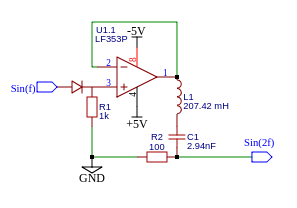
\includegraphics[width=0.6\textwidth]{designnotater/DN3/SchematicCRKT.png} 
  \caption{Realisering hvor dioden får fram de harmoniske, OP-ampen fungerer som en buffer mens kondensatoren og spolen danner et bånpassfilter.}
  \label{fig:Multiplikator}
\end{figure}

Filteret i seg selv testes ved bruk av en network- og spectrum analyser. Resultatene av dette er plottet i figur \ref{fig:netwok} og \ref{fig:bode}.

\begin{figure}[H]
  \centering
  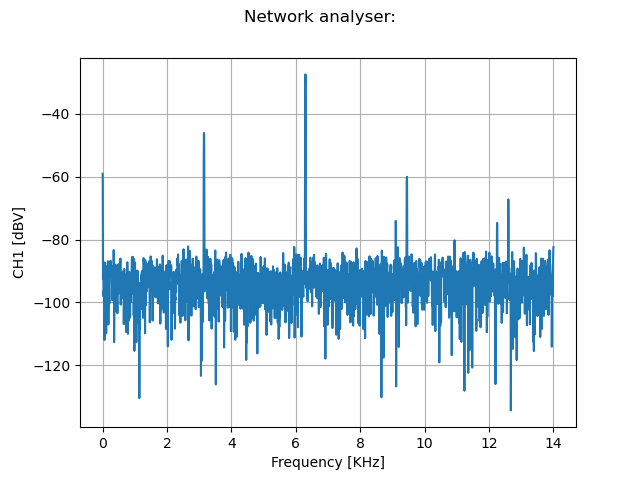
\includegraphics[width=1\textwidth]{TTT4260/DP3/network.png} 
  \caption{}
  \label{fig:netwok}
\end{figure}

\begin{figure}[H]
  \centering
  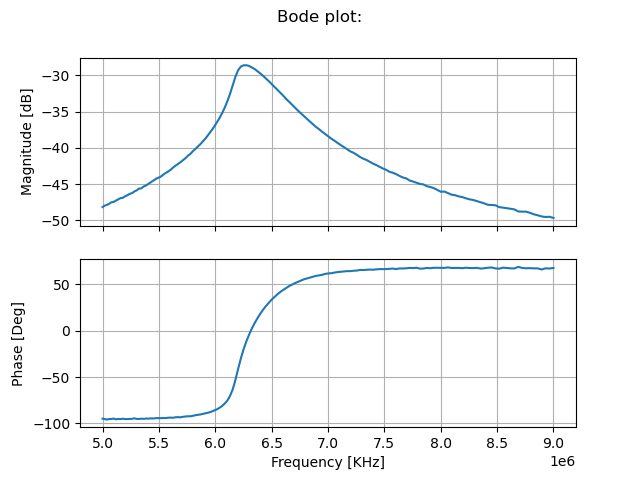
\includegraphics[width=1\textwidth]{TTT4260/DP3/Figure_1.png} 
  \caption{}
  \label{fig:bode}
\end{figure}

Teoretisk Q faktor er regnet ved formel \ref{eq:QRLC} og blir 84. Denne blir relativt høy fordi det er valgt en høy spoleverdi, samt lav motstandsverdi. Den fysiske oppkoblingen ser slik ut:

\begin{figure}[H]
  \centering
  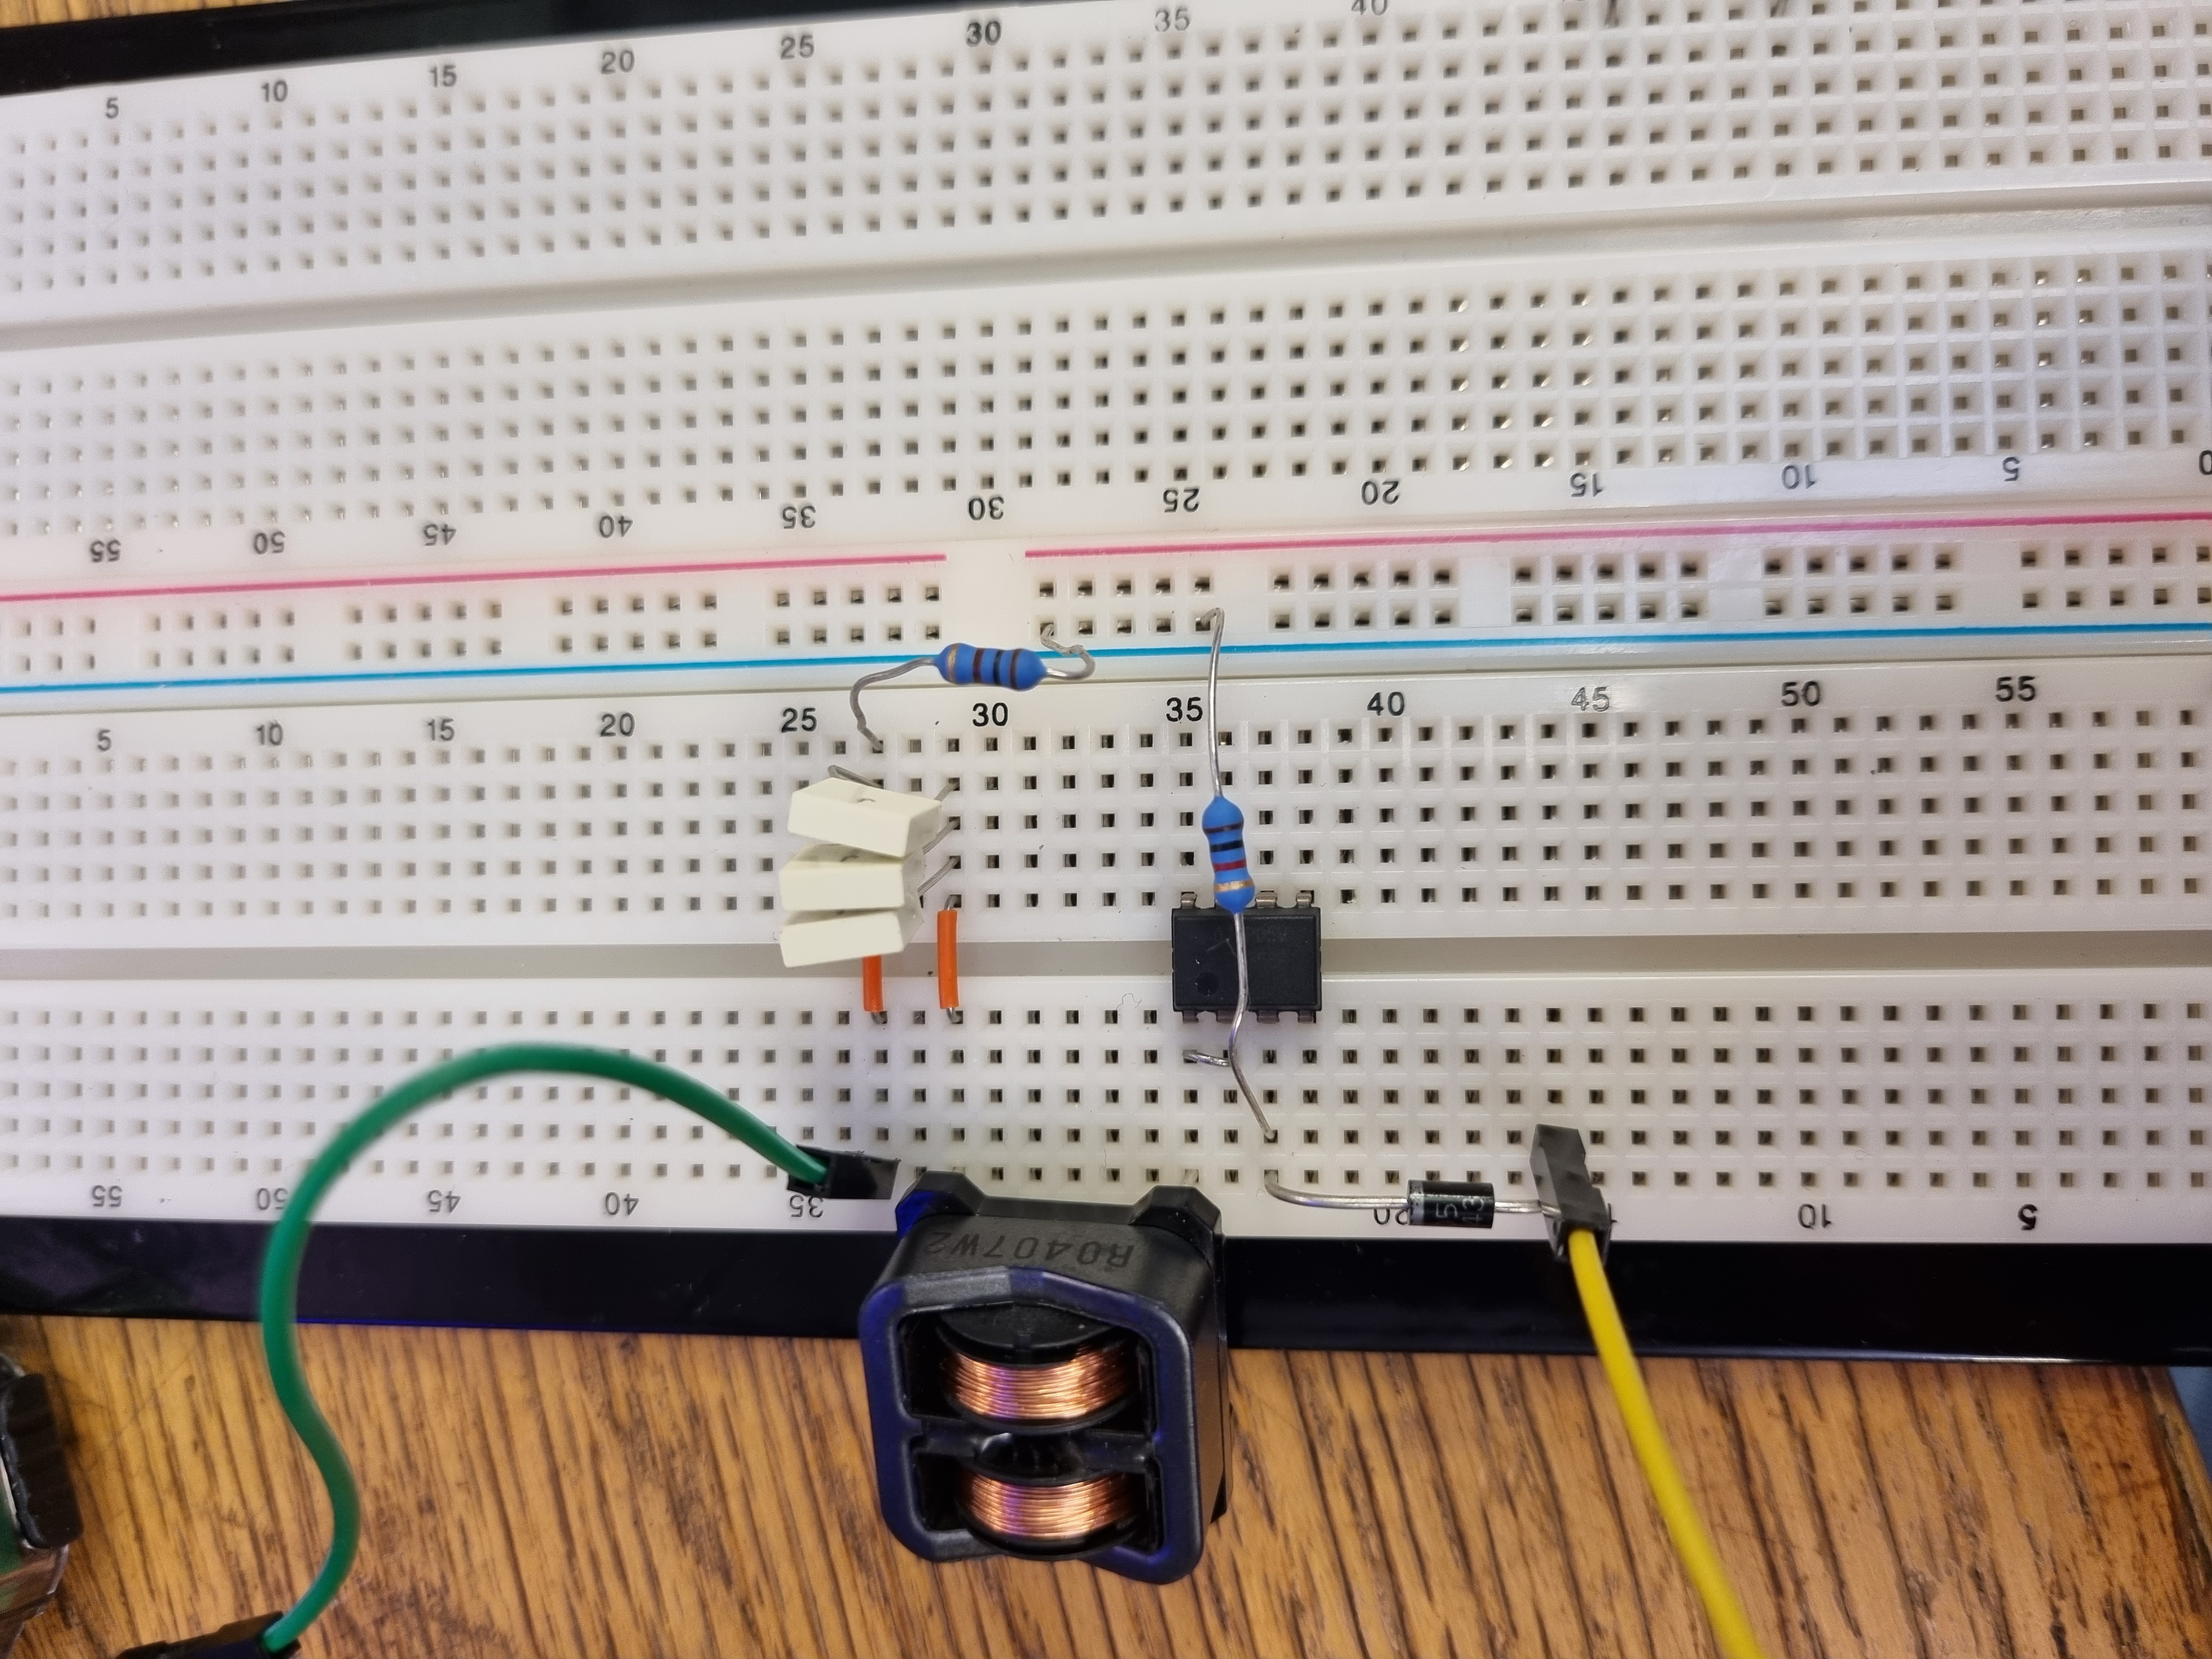
\includegraphics[width=0.6\textwidth]{TTT4260/DP3/20220322_193442.jpg} 
  \caption{Sinus inn i gul, sinus ut i grønn.}
  \label{fig:Fysisk}
\end{figure}

Ved hjelp av funksjonsgeneratoren påføres en sinus med frekvens 3.150 KHz, det måles v.ha. oscilloskopet en utgansfekvens på 6.34 KHz. Inn og ut signalet er tegnet i samme graf i figur \ref{fig:Skop}.

\begin{figure}[H]
  \centering
  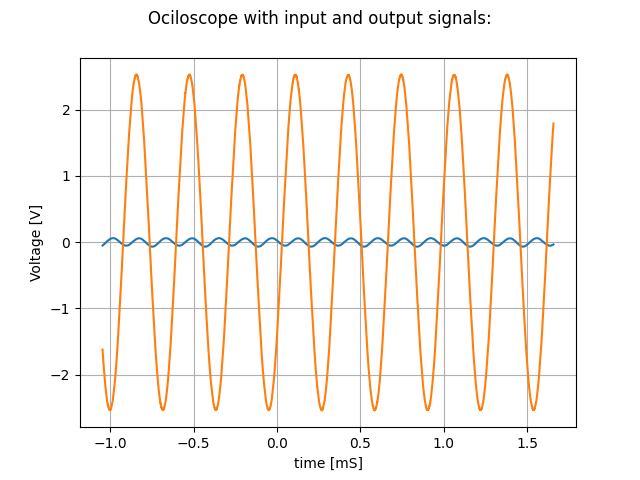
\includegraphics[width=1\textwidth]{TTT4260/DP3/ScopeOut.png} 
  \caption{Sinus inn i oransj, sinus ut i blått.}
  \label{fig:Skop}
\end{figure}


\section{Konklusjon}
\label{sec:konklusjon}

Systemet virker som forventet, men er er av dårlig kvalitet. Ut ifra spectrum-analyseren er den tydeligste responesen ved den ønskede frekvensen, men at det også er en ganske stor respons på de harmoniske. Grunnlaget for at de andre harmoiske ikke ble fjernet er kvaliteten på båndpass filteret bode-plottet viser til en depming på 20 dB.

For å forbedre designet kan det introduseres et forsterkningstrinn, samt flere båndpassfilter i serie.

\section{Takk}
Omega verksted for å fasitlitere prototyping.

%Bibliografi: Legg til flere elementer ved å legge til flere \bibitem:--------
\newpage
\phantomsection
\addcontentsline{toc}{section}{Referanser}
\begin{thebibliography}{99}

\bibitem{TekniskNotat}
  Lars	Lundheim,
  \emph{Teknisk notat: Frekvensmultiplikator},
  NTNU,
  1.1 versjon,
  Elsys-2021-LL-1,
  2021.

\bibitem{Hjelpehefte}
  Lars	Lundheim,
  \emph{Eit hjelpehefte: Innføring i analog og digital elektronikk},
  NTNU IES,
  2.1. versjon,
  2021.

\end{thebibliography}

\phantomsection
\addcontentsline{toc}{section}{Vedlegg}
\appendix
\label{sec:Vedlegg}
data.zip
%Tillegg. Flere tillegg legges til ved å lage flere sections:-----------------









\end{document}